\documentclass[slovene,11pt,a4paper]{article}
\usepackage[margin=2cm,bottom=2cm,foot=1.5cm]{geometry}
% \documentclass[slovene,11pt,a4paper]{article}
% \usepackage[margin=1.7cm,bottom=3cm,foot=1.5cm]{geometry}
\setlength{\parindent}{0pt}
\setlength{\parskip}{0.5ex}

\usepackage[pdftex]{graphicx}
\usepackage{pgffor}
\usepackage{subcaption}
% \usepackage{a4wide} %najaci package
\usepackage[utf8]{inputenc}
\usepackage[slovene]{babel}
\usepackage{color}
\usepackage{graphicx}
% \usepackage{subfigure}
\usepackage{imakeidx}
\usepackage{adjustbox}
\usepackage{float}
\usepackage{amsmath}
\usepackage{mathtools}
\usepackage{tikz}
\usepackage{amssymb}
\usepackage{listings}
\usepackage{siunitx}
\usepackage{hyperref}
\usepackage{amsfonts}
\usepackage{mathrsfs}

\def\phi{\varphi}
\def\eps{\varepsilon}
% \def\vartheta{\vartheta}

\newcommand{\thisyear}{2024/25}

\renewcommand{\Re}{\mathop{\rm Re}\nolimits}
\renewcommand{\Im}{\mathop{\rm Im}\nolimits}
\newcommand{\Tr}{\mathop{\rm Tr}\nolimits}
\newcommand{\diag}{\mathop{\rm diag}\nolimits}
\newcommand{\dd}{\,\mathrm{d}}
\newcommand{\ddd}{\mathrm{d}}
\newcommand{\ii}{\mathrm{i}}
\newcommand{\lag}{\mathcal{L}\!}
\newcommand{\ham}{\mathcal{H}\!}
\newcommand{\four}[1]{\mathcal{F}\!\left(#1\right)}
\newcommand{\bigO}[1]{\mathcal{O}\!\left(#1\right)}
\newcommand{\sh}{\mathop{\rm sinh}\nolimits}
\newcommand{\ch}{\mathop{\rm cosh}\nolimits}
\renewcommand{\th}{\mathop{\rm tanh}\nolimits}
\newcommand{\erf}{\mathop{\rm erf}\nolimits}
\newcommand{\erfc}{\mathop{\rm erfc}\nolimits}
\newcommand{\sinc}{\mathop{\rm sinc}\nolimits}
\newcommand{\rect}{\mathop{\rm rect}\nolimits}
\newcommand{\ee}[1]{\cdot 10^{#1}}
\newcommand{\inv}[1]{\left(#1\right)^{-1}}
\newcommand{\invf}[1]{\frac{1}{#1}}
\newcommand{\sqr}[1]{\left(#1\right)^2}
\newcommand{\half}{\frac{1}{2}}
\newcommand{\thalf}{\tfrac{1}{2}}
\newcommand{\pd}{\partial}
\newcommand{\Dd}[3][{}]{\frac{\ddd^{#1} #2}{\ddd #3^{#1}}}
\newcommand{\Pd}[3][{}]{\frac{\pd^{#1} #2}{\pd #3^{#1}}}
\newcommand{\avg}[1]{\left\langle#1\right\rangle}
\newcommand{\norm}[1]{\left\Vert #1 \right\Vert}
\newcommand{\braket}[2]{\left\langle #1 \vert#2 \right\rangle}
\newcommand{\obraket}[3]{\left\langle #1 \vert #2 \vert #3 \right \rangle}
\newcommand{\hex}[1]{\texttt{0x#1}}

\renewcommand{\iint}{\mathop{\int\mkern-13mu\int}}
\renewcommand{\iiint}{\mathop{\int\mkern-13mu\int\mkern-13mu\int}}
\newcommand{\oiint}{\mathop{{\int\mkern-15mu\int}\mkern-21mu\raisebox{0.3ex}{$\bigcirc$}}}

\newcommand{\wunderbrace}[2]{\vphantom{#1}\smash{\underbrace{#1}_{#2}}}

\renewcommand{\vec}[1]{\overset{\smash{\hbox{\raise -0.42ex\hbox{$\scriptscriptstyle\rightharpoonup$}}}}{#1}}
\newcommand{\bec}[1]{\mathbf{#1}}


\title{
\sc\large Matematično-fizikalni praktikum \thisyear \\
\bigskip
\bf\Large 7.~naloga: Newtonov zakon
}
\author{Tadej Tomažič}
\date{}

\makeindex[columns=3, title=Alphabetical Index, intoc]

\begin{document}


\pagenumbering{gobble} 
\author{Tadej Tomažič}
\date{\today}

\maketitle

\newpage
\pagenumbering{arabic}
\tableofcontents
\listoffigures
\newpage
\section{Navodila}


Gibanje masne točke v polju sil v eni dimenziji opišemo
z diferencialno enačbo drugega reda, z Newtonovim zakonom
\begin{equation*}
m\, \Dd[2]{x}{t} = F \>.
\end{equation*}
Enačba je seveda enakovredna sistemu enačb prvega reda
\[
m\, \Dd{x}{t} = p \;, \qquad \Dd{p}{t} = F
\]
in tako jo tudi rešujemo: kot sistem dveh enačb prvega reda.

Seveda morajo biti na voljo tudi ustrezni začetni pogoji, tipično
$x(t=0)=x_0$ in $dx/dt=v(t=0)=v_0$. Splošnejše gre tu za sistem diferencialnih
enačb drugega reda:
\[
\Dd[n]{y}{x} = f(x,y,y',y'',...),
\]
ki ga lahko prevedemo na sistem enačb prvega reda z uvedbo novih spremenljivk v slogu
gibalne količine pri Netwonovi enačbi ($y'=v,y''=z,...$).

Z nekaj truda se da eksplicitno dokazati, mi pa lahko privzamemo, da so metode za
reševanje enačb hoda (Runge-Kutta 4. reda, prediktor-korektor... ) neposredno uporabne
za reševanje takšnih sistemov enačb in torej aplikabilne v poljubno dimenzijah, kar
naj bi v principu zadovoljilo večino naših zahtev.

Obstaja še posebna kategorija tako imenovanih \emph{simplektičnih} metod, za enačbe, kjer je $f$ le funkcija koordinat, $f(y)$, ki (približno) ohranjajo tudi Hamiltonian,
torej energijo sistema. Najbolj znana metoda je Verlet/St\"ormer/Encke metoda, ki je globalno
natančna do drugega reda in ki točno ohranja tudi vrtilno količino sistema (če je ta v danem problemu smiselna). Rešujemo torej za vsak diskretni korak $n$ velikosti $h$, $x_n=x_0+n \cdot h$:
\[
\Dd[2]{y}{x} = f(y)
\]
in pri diskretizaciji dobimo recept za korak $y_n$ in $v_n=y'_n$:
\begin{eqnarray*}
y_{n+1} &=& y_n + h \cdot v_n + \frac{h^2}{2} \cdot f(y_n) \\
v_{n+1} &=& v_n +  \frac{h}{2} \cdot \left[ f(y_n) + f(y_{n+1}) \right].
\end{eqnarray*}
Alternativno lahko to shemo zapišemo tudi s pomočjo dodatnih vmesnih točk in preskakujemo med lego in hitrostjo z zamikom h/2 (od tod angleško ime 'leapfrog' za ta zapis):
\begin{eqnarray*}
y_{n+1} &=& y_n + h \cdot v_{n+1/2} \\
v_{n+3/2} &=& v_{n+1/2} + h \cdot f(y_{n+1}).
\end{eqnarray*}


V še enem drugačnem zapisu je metoda poznana tudi kot metoda ``Središčne razlike'' (Central Difference Method, CDM), če nas hitrost ne zanima:
\[
y_{n+1} - 2 y_n + y_{n-1} = h^2 \cdot f(y_n),
\]
kjer prvo točko $y_1$ izračunamo po originalni shemi. Metodo CDM lahko uporabljamo tudi
za primere, ko je f tudi funkcija 'časa' x, f(x,y), le da tu simplektičnost ni zagotovljena
(in tudi verjetno ne relevantna).
Za simplektične metode višjih redov je na voljo na primer Forest-Ruth metoda ali Position
Extended Forest-Ruth Like (PEFRL) metoda, ki sta obe globalno četrtega reda in enostavni za
implementacijo.

\bigskip

{\it Naloga\/}: Čim več metod uporabi za izračun
nihanja matematičnega nihala z začetnim pogojem  $\vartheta(0)= \theta_0 = 1$,$\dot{\vartheta}(0)=0$. 
Poišči korak, ki zadošča za natančnost na 3 mesta. Primerjaj
tudi periodično stabilnost shem: pusti, naj teče račun čez 10
ali 20 nihajev in poglej, kako se amplitude nihajev sistematično
kvarijo. Pomagaš si lahko tudi tako, da občasno izračunaš
energijo $E \propto  1-\cos \vartheta + \frac{\dot{\vartheta}^2 }{2 \omega_0^2} $. Nariši tudi
ustrezne fazne portrete!.
Z analitično rešitvijo dobimo za nihajni čas $\frac{4}{\omega_0} K\left(\sin^2\frac{\theta_0}{2}\right)$, kjer je $K(m)$ popolni
eliptični integral prve vrste, ki je v SciPy knjižnici in v članku na spletni učilnici podan z:
\[
K(m)=\int\limits_{0}^{1} \frac{d z}{\sqrt{\left(1-z^{2}\right)\left(1-m z^{2}\right)}} = \int\limits_{0}^{\frac{\pi}{2}} \frac{d u}{\sqrt{\left(1-m \sin^2{u}\right)}}
\] 
Previdno, obstaja tudi definicija z $m^2$ v integralu - potem je prav $K\left(\sin\frac{\theta_0}{2}\right)$, brez kvadrata (npr že v Wikipediji)!
%K(\sin 0.5) = 1.67499$. 

(Dodatno lahko tudi
sprogramirate eliptični integral, ki je analitična rešitev
dane enačbe ali pa ga vzamete iz ustreznih programskih knjižnjic).

\bigskip

{\it Dodatna naloga\/:} Razišči še resonančno krivuljo
vzbujenega dušenega matematičnega nihala
\begin{equation*}
\Dd[2]{x}{t} + \beta\Dd{x}{t}+ \sin x = v\cos\omega_0t\>,
\end{equation*}
kjer je $\beta$ koeficient dušenja, $v$ in $\omega_0$ pa amplituda in
frekvenca vzbujanja.  Opazuj obnašanje odklonov in hitrosti nihala
pri dušenju $\beta=0.5$, vzbujevalni frekvenci $\omega_0=2/3$ in
amplitudo vzbujanja na območju $0.5 < v < 1.5$.
Poskusi opaziti histerezno obnašanje resonančne krivulje pri velikih amplitudah vzbujanja
(Landau, Lifšic, CTP, Vol.~1, {\sl Mechanics\/}).

\bigskip

{\it Dodatna dodatna naloga\/:} če ti gre delo dobro od rok,
si oglej še odmike in hitrosti (fazne portrete) van der Polovega oscilatorja
\begin{equation*}
\Dd[2]{x}{t} - \lambda\Dd{x}{t}
\left( 1 - x^2 \right) + x = v\cos\omega_0t
\end{equation*}
s parametri $\omega_0=1$, $v=10$ ter $\lambda=1$ ali $100$.
Tu se ne trudi s preprostimi diferenčnimi shemami: problem
je nelinearen in tog, zato uporabi neko preverjeno metodo
(na primer iz družine Runge-Kutta ali ekstrapolacijsko
metodo) s prilagajanjem velikosti koraka.
\section{Rešitev}

Najprej si poglejmo avtokorelacijo za obe sovi.
\begin{figure}[h]
    \centering
    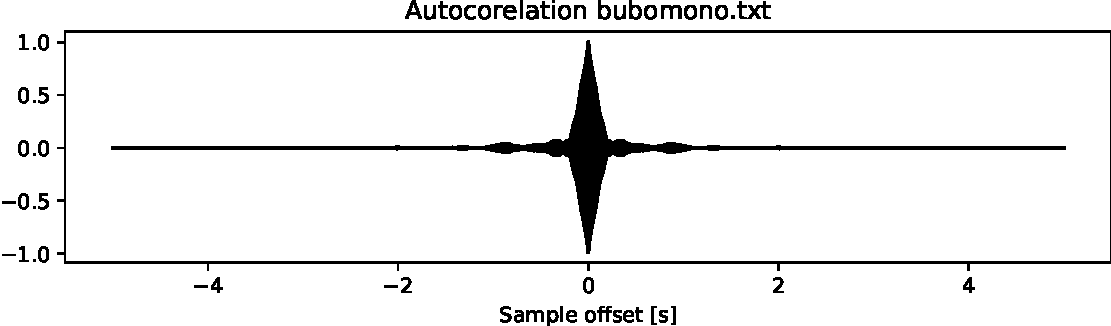
\includegraphics[width=12cm]{pdfs/bubomono.txt_acor.pdf}
    \vspace{10pt}
    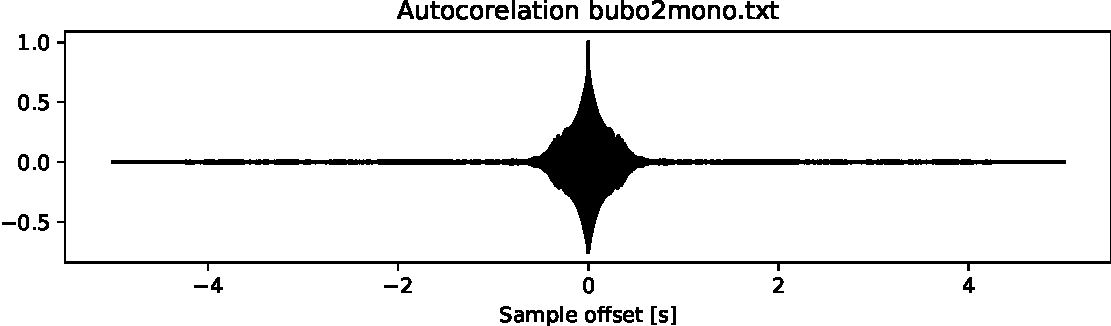
\includegraphics[width=12cm]{pdfs/bubo2mono.txt_acor.pdf}
    \caption{Avtokorelacija signala sov}
\end{figure}

Preden sem koreliral signal sem vektorja samplov normiral, tako da je
"najmočnejši" signal 1. To pomeni \[\|x\|_\infty = \max_i |x_i|\]

Poglejmo si še korelacije med sovami in posnetki:
\newpage
\begin{figure}[h]
    \centering
    \foreach \mix in {mix, mix1, mix2, mix22} {
        \foreach \sova in {bubomono, bubo2mono}{
            \includegraphics[width=8cm]{pdfs/cor_\mix.txt_\sova.txt.pdf}
        }
    }
    \caption{Korelacija sov in posnetkov iz narave}
\end{figure}
Tukaj je bila normalizacija drugače izbrana. Tukaj je bila narejena normalizacija korelacije. Če je varianca signala a $\sigma_a$,
potem je $ \mathbf{x} = \mathbf{x} / \left(\sigma_a \sigma_b |\mathbf{b}|\right)$. Sigma je izračunana z \verb|numpy.std()|.


Hitrosti so precej dolgčasno pričakovane ampak vseeno.
\begin{figure}[h]
    \centering
    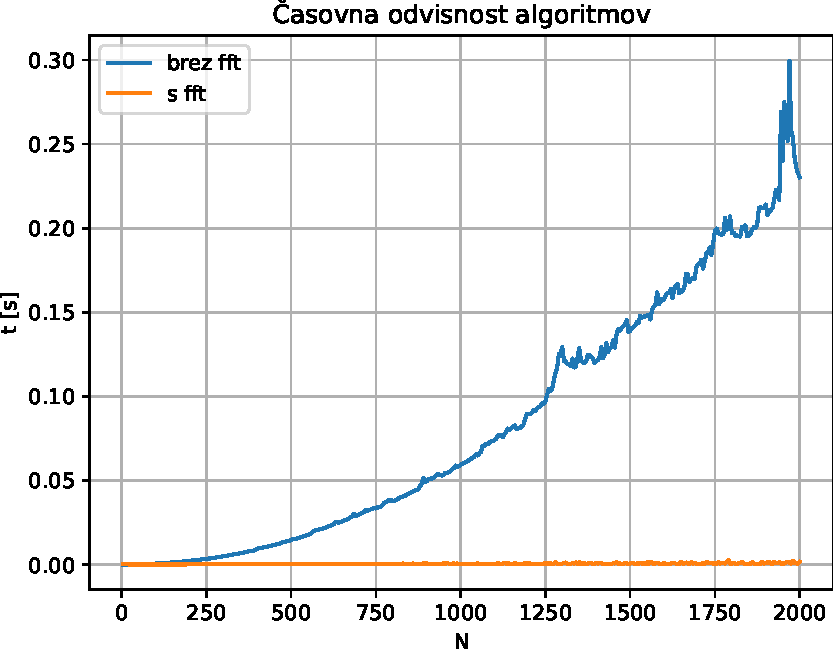
\includegraphics[width=8cm]{pdfs/cas-lin.pdf}
    \vspace{10pt}
    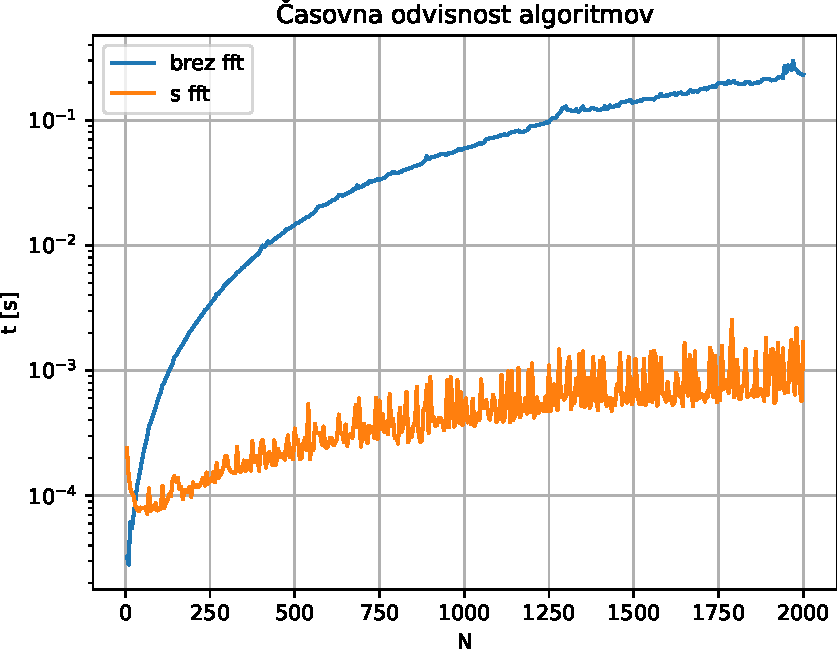
\includegraphics[width=8cm]{pdfs/cas-log.pdf}
    \caption{Hitrost algoritmov}
\end{figure}
\newpage
\section{Dodatna naloga}
Posnel sem dva človeka m in ž ko izgovarjata aaaaaaaaaaaa. Posnel sem jih tudi
ko bereta slovar. Gledal sem ali lahko spet zaznam ali gre za ž glas ali m glas.
Poglejmo si spektra njunega glasu.
\begin{figure}[h]
    \begin{center}
        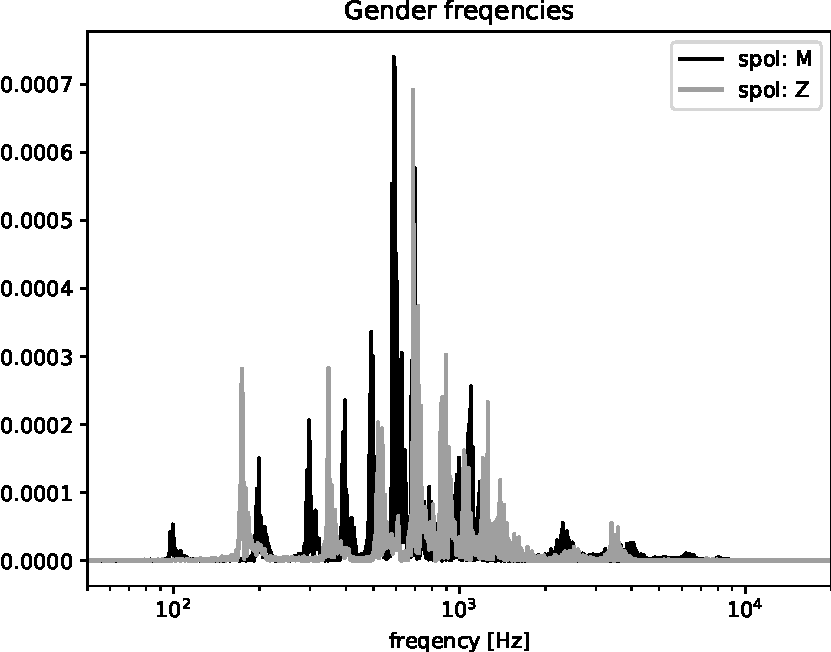
\includegraphics[width=12cm]{pdfs/fft_spol.pdf}
    \end{center}
    \caption{Barva glasu moškega in ženske}
\end{figure}

% Glasova sta bila prej normirana, saj je bil moški glas posnet bližje mikrofona.
% Poglejmo si zopet korelacijo med posnetki:
% \foreach \gender in {Z, M} {
%     \foreach \mix in {Glas\ 001, Glas\ 002}{
%         pdfs/cor_\gender_\mix.pdf 
%     }
% }
\begin{figure}[h]
    \begin{center}
        
    \foreach \gender in {Z, M} {%
        \foreach \mix in {001, 002} {%
            \includegraphics[width=8cm]{pdfs/cor_\gender_Glas\space\mix.pdf}%    
        }%
        \par
}%
    \end{center}
    
    \caption{Korelacija glasa človeka in posnetkov iz branja slovarja}
\end{figure}
\end{document}
